% --------------------------------------------------------------------------------
% Concepts: Introduction
% --------------------------------------------------------------------------------

% --------------------------------------------------------------------------------
\chapter{Introduction}
% --------------------------------------------------------------------------------

The toolbox is a collection of MATLAB \emph{functions} for
perception-based music analysis. These "building blocks" are
combined to form \emph{modules}, related to musical perceptual
phenomena, which will be described in the following chapter. The
next chapter will evaluate some of these modules with respect to
data from psychoacoustical experiments. In a subsequent chapter
these modules are then used in some applications to demonstrate
their effectiveness.

The modules are described from different points of view so that
you can access them at different levels. We offer you an
introductory, functional-logical, signal processing,
implementation, and example-based description.
\begin{enumerate}
\item
    The \emph{introductory description} provides just a simple verbal
    description of what the module does, how it is situated in our
    global conception, what the inputs are and what outputs are generated.
\item
    The \emph{functional-logical description}
    allows a concise description which resembles the way in
    which the MATLAB functions are to be used while programming in MATLAB.
    The approach is vector oriented (see next paragraph).
\item
    The \emph{signal processing description} gives a mathematical
    description of the modules in terms of a functional
    equivalence model of physiological processes. A trade-off had
    to be found between psychoacoustical and physiological
    accurateness and processing efficiency. Our approach is based
    on filter theory and vector processing rather than physical
    modeling.
    \footnote{An essential aspect, for example, concerns the
    auditory peripheral part. Rather than having a physical model
    of the resonance of the basilair membrane and subsequent hair
    cells in response to sound, the effects of the cochlear
    hydromechanics and hair cells are simulated by means of an
    array of overlapping (asymmetric) band-pass filters and
    subsequent non-linear transformation into neural firing
    rate-code (not firing spike-code).}
\item
    The \emph{implementation description} concerns the way in
    which the MATLAB functions are implemented.
    Signal processing functions of the MATLAB signal processing toolbox have
    been used where possible.
    See the \hyperlink{Part:ReferenceManual}{Reference Manual}
    for more details on the implemented MATLAB functions.
\item
    Finally for each module we also provide a number of
    \emph{examples}.
\end{enumerate}

There is another important thing that you should know. The modules
are related to auditory information processing. That means: we
start from sound and transform sounds into either auditory images
or inferences. \emph{Auditory images}, or images in short, reflect
features of the sound as internal representations, in other words
as brain activations so to speak. \emph{Inferences}, on the other
hand, provide derived information that can be compared to human
behavior.

Hence our dual validation model: images and associated processes
are compared with human physiology, while inferences are compared
with human behavioral responses (fig.
\ref{Fig:ConceptualFramework}). This is why we introduce the
following important notions in our approach, which define our
global internal representational framework:
\begin{itemize}
\item
    An \emph{image} has two aspects: (i) its content represents
    features related to the musical signal, and (ii) it is assumed
    to be carried by an array of neurons. From the point of view
    of computer modeling, an image is an ordered array of numbers
    (= a vector) whose values represent neural activation. We
    conceived of neural activation in terms of firing
    \emph{rate-code}, that is, the probability of neuronal spiking
    during a certain time interval. Hence images are to be
    conceived of as snapshots of the brain activation (or better:
    what we believe to be snapshots of brain activation). A
    distinction will be made between different types of images
    (such as \emph{primary} images, \emph{pitch} images,
    \emph{spectral} images, etc...). A main characteristic and
    limitation of our current state-of-the-art is that images are
    basically \emph{frame based}. In other words, we do not yet
    consider an \emph{object-based} representation of musical
    content.
\item
    Processes dealing with image transformations are called
    \emph{image transformation processes}. They transform sounds
    into images, and images into other images. This is a good
    place to say that different memory systems carry different
    kinds of images, hence our inclination to speak about
    short-term images and long-term images in association with
    short-term memories and long-term memories.
\item
    \emph{Inferences} are outputs that can be directly compared
    with listener's behavioral responses to musical information
    processing.
\item
    \emph{Inference processes} compare images, inspect images or
    extract features from images.
\end{itemize}

Figure \ref{Fig:ConceptualFramework} gives an overview of the
internal representational framework.
\begin{figure}[h]
    \centering
    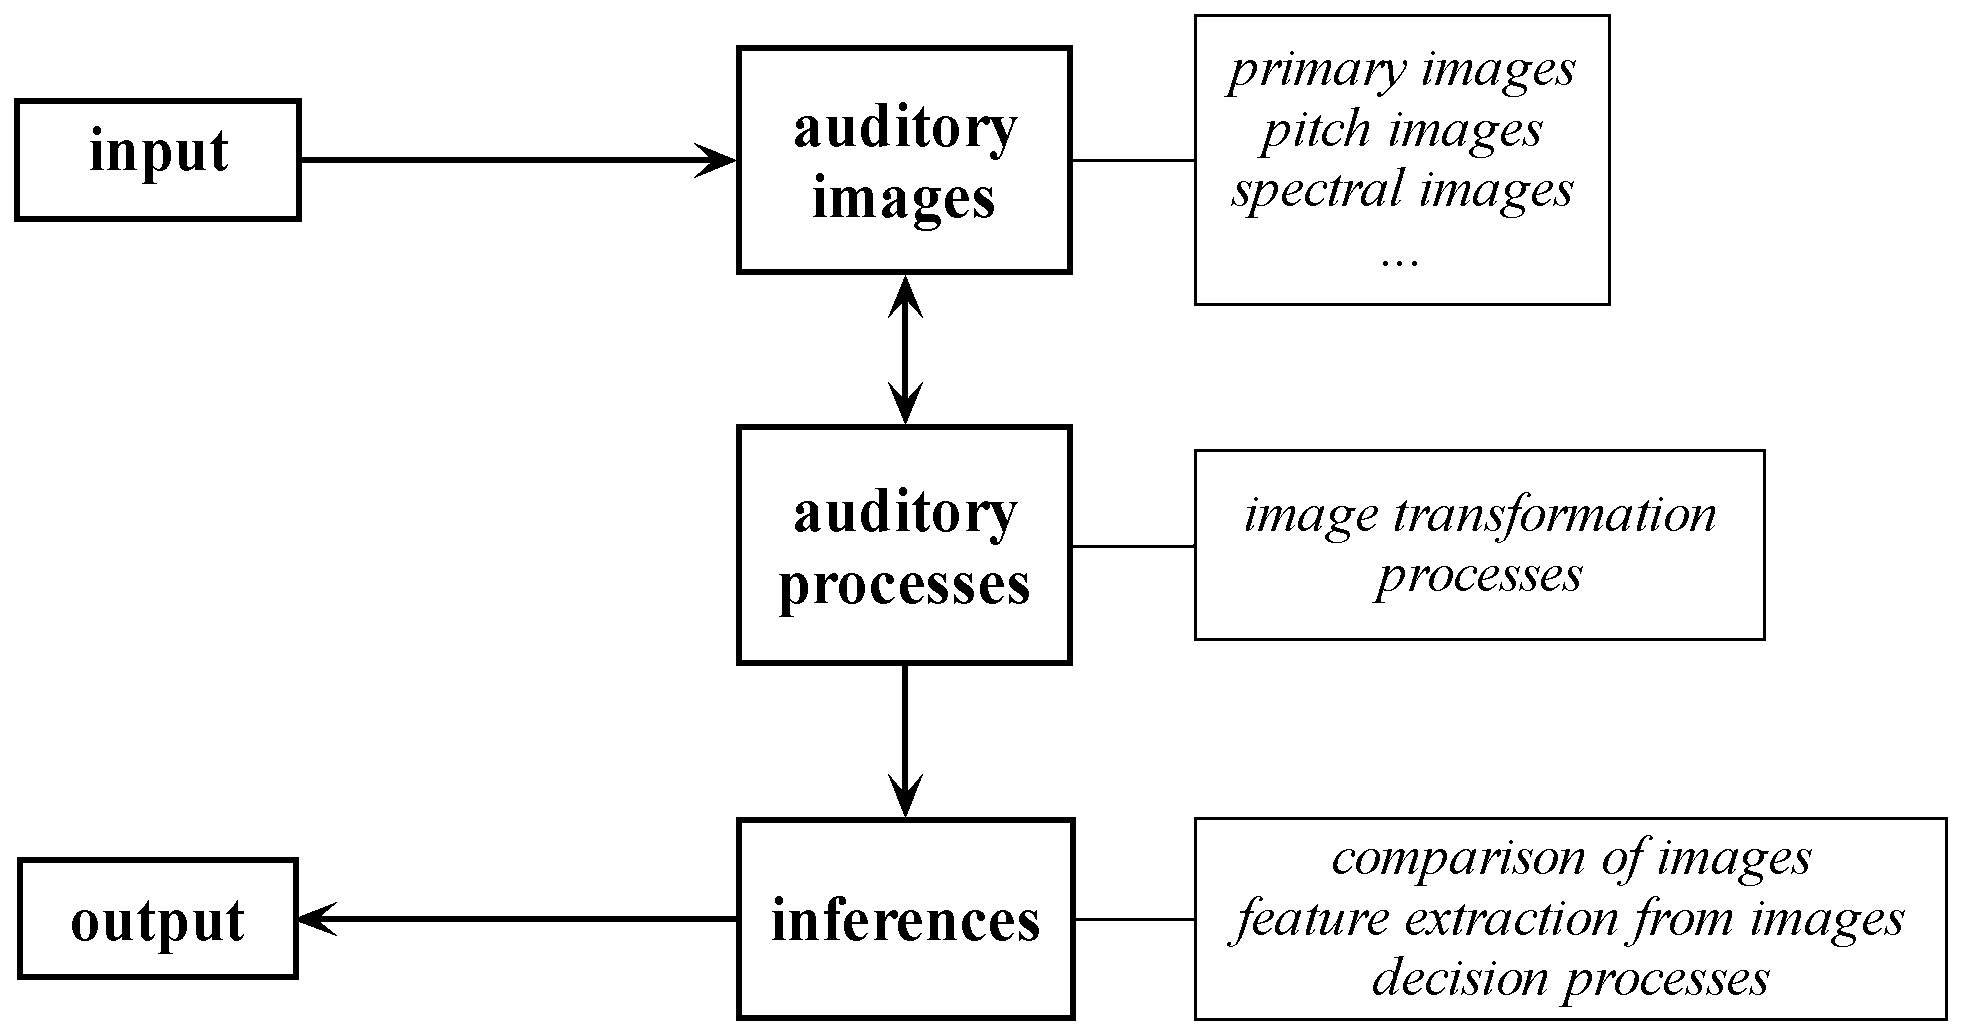
\includegraphics[width=\IPEMDefaultFigureWidth]{Graphics/ConceptualFramework}
    \caption{Overview of the internal representational framework.}
    \label{Fig:ConceptualFramework}
\end{figure}
